\section{Les concepts de base}
\subsection{Les fichiers}


\begin{frame}{Les fichiers}

    \begin{center}
        \includegraphics[height=3cm]{compilation.jpg}
    \end{center}
    \begin{itemize}
        \item Fichier source = essais\alert{\textbf{.tex}}
        \item Fichier de bibliographie = essais\alert{\textbf{.bib}}
        \item Lors de compilation $\rightarrow$ création de nombreux fichiers annexes
        \begin{itemize}
            \item style, class;
            \item structure du document;
            \item table des matières, liste des figures;
            \item liste des références;
            \item \ldots{}
        \end{itemize}
        \item Création d'un fichier essais\alert{\textbf{.pdf}}
    \end{itemize}

\end{frame}

%-----------------------

\subsection{La structure du fichier}

\begin{frame}[fragile,label=frame:structure]{Structure générale du document I}

  \framesubtitle{Document minimal}
  \small

  \begin{lstlisting}[style=nonumbers]
  \documentclass{article} %Type de document

  %Préambule
  %On charge ici les packages

  \begin{document}
      %Corps du document
  \end{document}
  \end{lstlisting}
  \begin{itemize}
      \item On charge les \textit{packages} et effectue certains réglages dans le préambule.
      \item On écrit le contenu de son document entre \lstinline|\begin{document}| et \lstinline|\end{document}|.
      \item Commentaires introduits par \%
  \end{itemize}

\end{frame}

\begin{frame}[fragile]{Structure générale du document II}

  \framesubtitle{Exemple de document type}
  \small
  \begin{tabular}{ll}
    Type de document &
    \lstinline|\documentclass[a4paper, 10pt]{scrartcl}|\\
    Utilisation de \textit{package} &
    \lstinline|\usepackage[utf8]{inputenc}|\\
    Utilisation de \textit{package} &
    \lstinline|\usepackage[T1]{fontenc}|\\
    Utilisation de \textit{package} &
    \lstinline|\usepackage[french]{babel}|\\
     &\\
    Début du document &
    \lstinline|\begin{document}|\\
    Corps du document &
    \lstinline|Ceci est mon premier document en Latex !!!|\\
    Fin du document &
    \lstinline|\end{document}|\\
  \end{tabular}
\end{frame}

\subsection{Commandes et environnements}
\begin{frame}[fragile]{Les Commandes}
  \begin{itemize}
  \item \textbf{Commande}
      \begin{itemize}
      \item Débute par \textbackslash
      \item Peut prendre plusieurs arguements, placés entre accolades
      \item Permet d'insérer des symboles
      \end{itemize}
      \begin{lstlisting}[style=nonumbers]
  \commandName[options]{FirstParameter} ... {LastParameter}
      \end{lstlisting}
      \begin{center}
      \begin{tabular}{lllll}
      \lstinline|\implies| & $\implies$ & & \lstinline|\textbf{texte}| & \textbf{texte}
      \end{tabular}
      \end{center}
  \end{itemize}
\end{frame}

\begin{frame}[fragile]{Les Environnements}
  \begin{itemize}
  \item \textbf{Environnement}
      \begin{itemize}
      \item S'applique à des \textit{portions de texte} et permet par exemple d'appliquer une règle de mise en page
      \item Délimité par \lstinline|\begin{}| et \lstinline|\end{}|
      \end{itemize}
      \begin{lstlisting}[style=nonumbers]
  \begin{EnvironnementName}[options]

  \end{EnvironnementName}
      \end{lstlisting}
      \begin{center}
        \begin{columns}
        \begin{column}{0.5\textwidth}
        \begin{lstlisting}[style=nonumbers]
  \begin{figure}
      \centering
      
\includegraphics{logo-uclouvain.eps}
      \caption{Voici le logo UCLouvain}
      \label{fig:ucl}
  \end{figure}
        \end{lstlisting}
        \end{column}
        \begin{column}{0.5\textwidth}
        \begin{figure}[!ht]
            \centering
            
\includegraphics[width=0.50\textwidth]{logo-uclouvain.pdf}
            \caption{Voici le logo UCLouvain}
            \label{fig:ucl}
        \end{figure}
        \end{column}
        \end{columns}
      \end{center}
  \end{itemize}
\end{frame}

%-----------------------

\subsection{Les classes}

\begin{frame}[fragile]{Les principales classes de document}
  \begin{tabular}{p{0.2\textwidth}p{0.8\textwidth}}
    \textbf{scrartcl} & pour les articles de journaux scientifiques, présentations, rapports courts,\dots \\ \\
    \textbf{scrreprt} & pour de plus long rapports de plusieurs chapitres, petits livres, thèses,\dots \\ \\
    \textbf{beamer} & pour écrire des présentations (comme celle-ci) \\ \\
    \textbf{et beaucoup d'autres} & dont les références sont facilement trouvables sur Internet
  \end{tabular}
  %\vspace{1cm}
  \begin{center}
  \verb|\documentclass[a4paper,10pt]{|\alert{\texttt{scrartcl}}\verb|}|\\
  \end{center}
\end{frame}

\subsection{Les options}

\begin{frame}[fragile]{Les principales options de document}
  \begin{tabular}{lp{8cm}}
    \textbf{10pt, 11pt, 12pt} & pour la taille de police.\\
    \textbf{a4paper, a5paper} & pour la taille de page.\\
    \textbf{twoside} & pour des marges de livre
  \end{tabular}
  \vspace{1cm}
  \begin{center}
  \verb|\documentclass[|\alert{\texttt{a4paper,10pt}}\verb|]{scrartcl}|\\
  \end{center}
\end{frame}

\subsection{Les packages}

\begin{frame}[fragile]{Les packages}
  \begin{itemize}
  \item Les \textbf{packages} sont des extensions contenant de nouveaux environnements et commandes
  \item Appel du package dans le \textit{préambule} à l'aide de la commande \lstinline|\usepackage[options]{packageName}|
  \end{itemize}
  \vskip2em
  \begin{tabular}{ll}
  \lstinline|\usepackage[utf8]{inputenc}| & Utilisation des caractères accentués \\
  \lstinline|\usepackage[T1]{fontenc}| & Permet d'utiliser tous les caractères du clavier \\
  \lstinline|\usepackage[french]{babel}| & Spécifie la langue (français ici) \\
  \lstinline|\usepackage{graphicx}| & Permet d'importer des images
  \end{tabular}
  \vskip2em
  \begin{itemize}
      \item Les 3 premiers packages de l'exemple sont nécessaires à la compilation !
  \end{itemize}
\end{frame}

\subsection{La structure du document}

\begin{frame}[fragile]{La structure logique du document}
    \begin{itemize}
        \item Structure logique du document uniquement
        \item \LaTeX{} se charge de la numérotation et de la mise en page\\
    \end{itemize}
    \vspace{1cm}

    \begin{itemize}
        \item \lstinline|\section{}|
        \item \lstinline|\subsection{}|
        \item \lstinline[mathescape]|\$\color{blue}{\texttt{paragraph}}${}| % Don't question it, it just works
    \end{itemize}

\end{frame}

\begin{frame}[fragile]{La structure logique du document}
  \framesubtitle{Exemple}
  \begin{columns}
    \begin{column}{0.5\textwidth}
      \begin{lstlisting}[style=nonumbers,mathescape]
\section{Une $\color{black}{\texttt{section}}$}
\subsection{Une sous-$\color{black}{\texttt{section}}$}
\paragraph{Un paragraph} Le contenu de mon paragraphe sans alinéa.

Un paragraphe sans titre.
La première ligne a toujours un alinéa.

Un deuxième paragraphe sans titre.
À nouveau la première ligne a un alinéa.
      \end{lstlisting}
    \end{column}
    \begin{column}{0.5\textwidth}
      \fbox{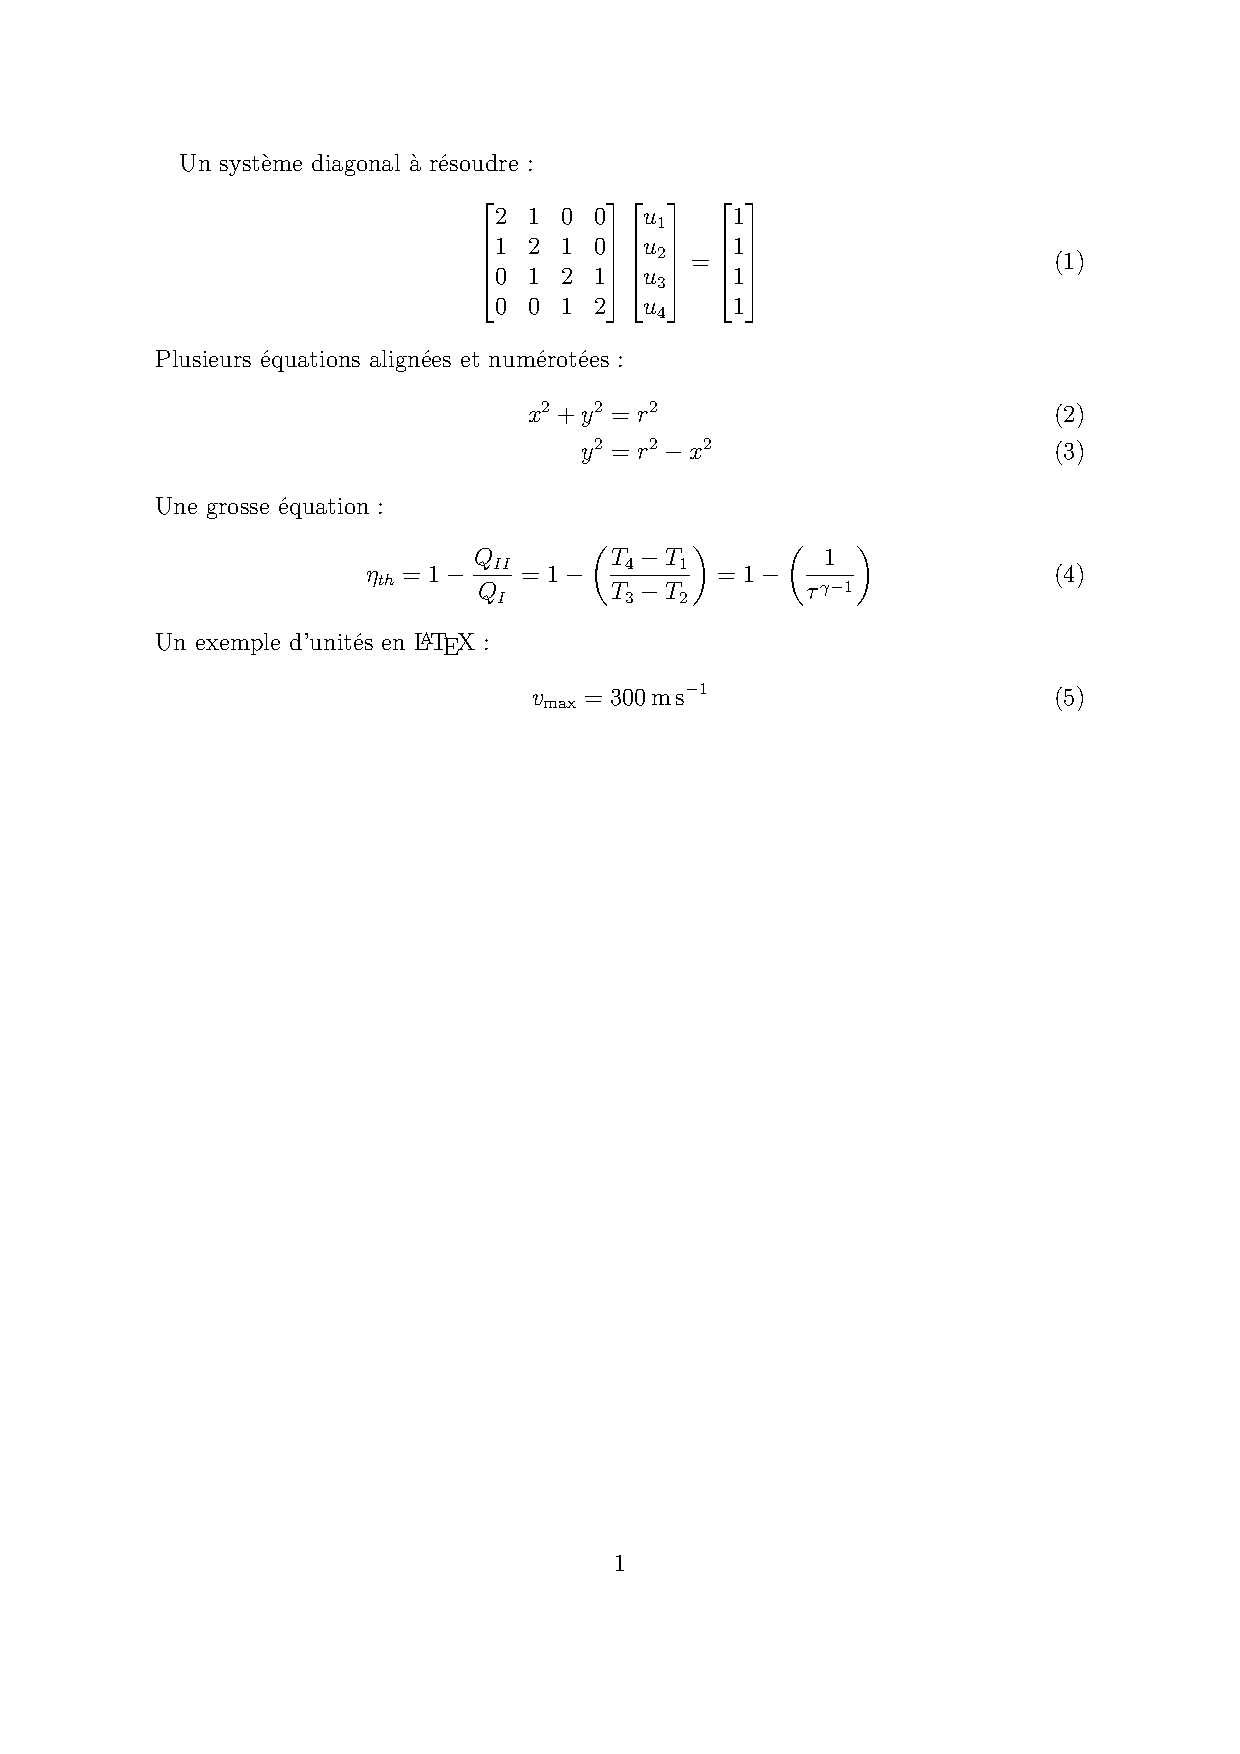
\includegraphics[width=1\textwidth,trim={1.5cm 14cm 1.5cm 1cm},clip]{examples/structure/build_latex/main.pdf}}
    \end{column}
  \end{columns}
  \begin{itemize}
  \item Pour créer un nouveau paragraphe, il suffit de faire deux retours à la ligne.
  \end{itemize}
\end{frame}
